\documentclass{standalone}
\usepackage{tikz, tipa}
\begin{document}
\tikzset{corres/.style={fill=white, right=6mm, above=1mm,inner sep=0pt}}
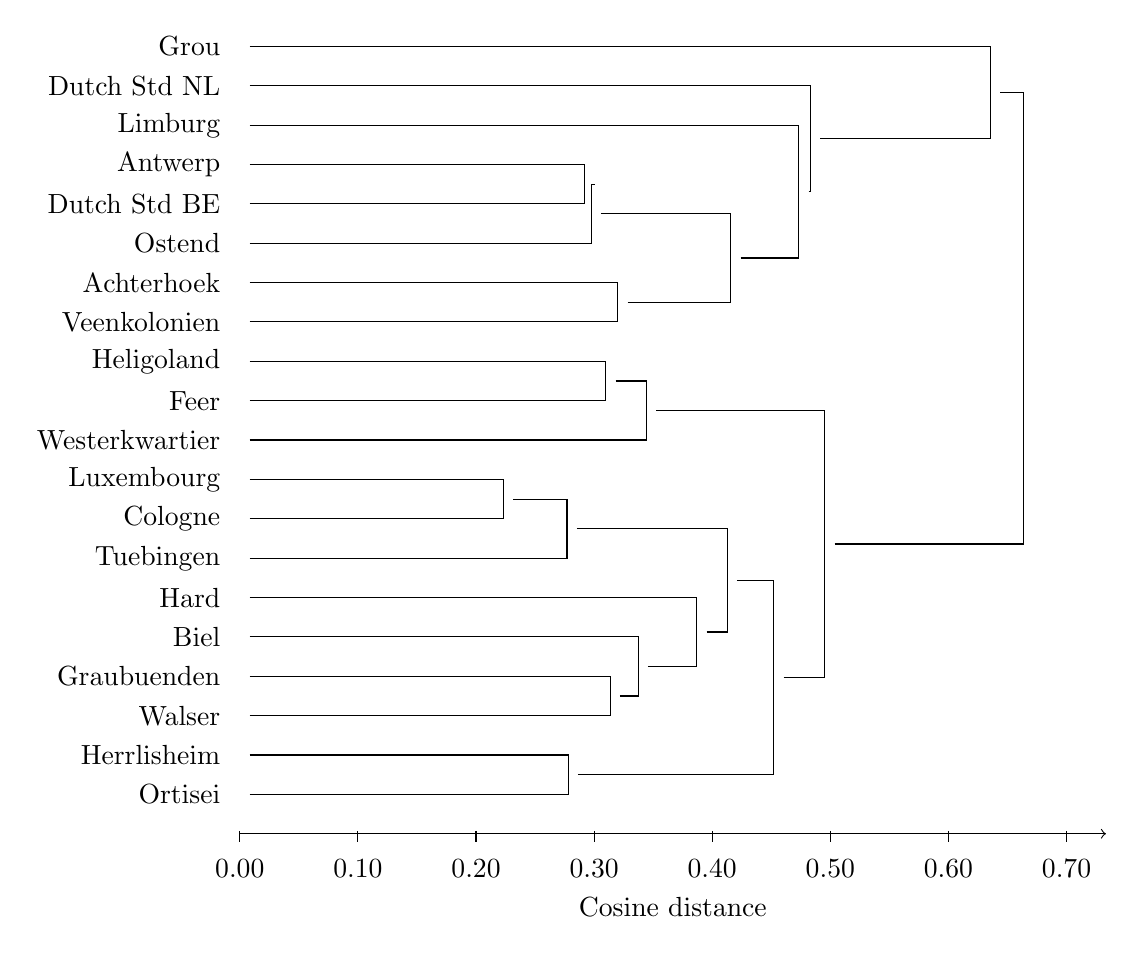
\begin{tikzpicture}
% Doculects by singleton cluster number (alphabetical index).
\node[label=left:Ortisei] (14) at (0, 0.5) {};
\node[label=left:Herrlisheim] (11) at (0, 1.0) {};
\node[label=left:Walser] (18) at (0, 1.5) {};
\node[label=left:Graubuenden] (7) at (0, 2.0) {};
\node[label=left:Biel] (2) at (0, 2.5) {};
\node[label=left:Hard] (9) at (0, 3.0) {};
\node[label=left:Tuebingen] (16) at (0, 3.5) {};
\node[label=left:Cologne] (3) at (0, 4.0) {};
\node[label=left:Luxembourg] (13) at (0, 4.5) {};
\node[label=left:Westerkwartier] (19) at (0, 5.0) {};
\node[label=left:Feer] (6) at (0, 5.5) {};
\node[label=left:Heligoland] (10) at (0, 6.0) {};
\node[label=left:Veenkolonien] (17) at (0, 6.5) {};
\node[label=left:Achterhoek] (0) at (0, 7.0) {};
\node[label=left:Ostend] (15) at (0, 7.5) {};
\node[label=left:Dutch Std BE] (4) at (0, 8.0) {};
\node[label=left:Antwerp] (1) at (0, 8.5) {};
\node[label=left:Limburg] (12) at (0, 9.0) {};
\node[label=left:Dutch Std NL] (5) at (0, 9.5) {};
\node[label=left:Grou] (8) at (0, 10.0) {};

% Clusters from Z.
\node (20) at (3.3480065271320134,4.25) {};
\draw (3) -| (20.center);
\draw (13) -| (20.center);
\node (21) at (4.1551842120250475,3.875) {};
\draw (16) -| (21.center);
\draw (20) -| (21.center);
\node (22) at (4.170576227834464,0.75) {};
\draw (11) -| (22.center);
\draw (14) -| (22.center);
\node (23) at (4.382427454237783,8.25) {};
\draw (1) -| (23.center);
\draw (4) -| (23.center);
\node (24) at (4.461481769539182,7.875) {};
\draw (15) -| (24.center);
\draw (23) -| (24.center);
\node (25) at (4.647878425660961,5.75) {};
\draw (6) -| (25.center);
\draw (10) -| (25.center);
\node (26) at (4.702382218040486,1.75) {};
\draw (7) -| (26.center);
\draw (18) -| (26.center);
\node (27) at (4.800780925110995,6.75) {};
\draw (0) -| (27.center);
\draw (17) -| (27.center);
\node (28) at (5.05956223173629,2.125) {};
\draw (2) -| (28.center);
\draw (26) -| (28.center);
\node (29) at (5.164958161850917,5.375) {};
\draw (19) -| (29.center);
\draw (25) -| (29.center);
\node (30) at (5.804666589012486,2.5625) {};
\draw (9) -| (30.center);
\draw (28) -| (30.center);
\node (31) at (6.190013781774778,3.21875) {};
\draw (21) -| (31.center);
\draw (30) -| (31.center);
\node (32) at (6.236986779567907,7.3125) {};
\draw (24) -| (32.center);
\draw (27) -| (32.center);
\node (33) at (6.7834899535005615,1.984375) {};
\draw (22) -| (33.center);
\draw (31) -| (33.center);
\node (34) at (7.098915085863936,8.15625) {};
\draw (12) -| (34.center);
\draw (32) -| (34.center);
\node (35) at (7.24714660380404,8.828125) {};
\draw (5) -| (35.center);
\draw (34) -| (35.center);
\node (36) at (7.429419506782082,3.6796875) {};
\draw (29) -| (36.center);
\draw (33) -| (36.center);
\node (37) at (9.533330945319397,9.4140625) {};
\draw (8) -| (37.center);
\draw (35) -| (37.center);
\node (38) at (9.951659863807546,6.546875) {};
\draw (36) -| (38.center);
\draw (37) -| (38.center);

% X axis.
\draw[->] (0,0) -- node[label={[label distance=-1.3cm]Cosine distance}]{{}} (11.0, 0);
\draw (0.0, 1pt) -- (0.0, -3pt) node[label={[label distance=-7mm]0.00}] {};
\draw (1.5, 1pt) -- (1.5, -3pt) node[label={[label distance=-7mm]0.10}] {};
\draw (3.0, 1pt) -- (3.0, -3pt) node[label={[label distance=-7mm]0.20}] {};
\draw (4.5, 1pt) -- (4.5, -3pt) node[label={[label distance=-7mm]0.30}] {};
\draw (6.0, 1pt) -- (6.0, -3pt) node[label={[label distance=-7mm]0.40}] {};
\draw (7.5, 1pt) -- (7.5, -3pt) node[label={[label distance=-7mm]0.50}] {};
\draw (9.0, 1pt) -- (9.0, -3pt) node[label={[label distance=-7mm]0.60}] {};
\draw (10.5, 1pt) -- (10.5, -3pt) node[label={[label distance=-7mm]0.70}] {};
\end{tikzpicture}
\end{document}
